\documentclass[11pt]{article}
\usepackage[margin=1in]{geometry}
\usepackage[T1]{fontenc}
\usepackage{lmodern}
\usepackage{microtype}
\usepackage{amsmath}
\usepackage{booktabs,tabularx,array}
\usepackage{enumitem}
\usepackage{xcolor}
\usepackage{listings}
\usepackage{tikz}
\usetikzlibrary{arrows.meta,positioning,calc}
\usepackage[obeyspaces,spaces]{url}
\usepackage[hidelinks]{hyperref}

\setlist{itemsep=2pt,topsep=4pt}
\setlength{\parskip}{4pt}
\setlength{\emergencystretch}{3em}
\renewcommand{\arraystretch}{1.2}
\newcolumntype{Y}{>{\raggedright\arraybackslash}X}

\definecolor{codebg}{RGB}{247,247,250}
\definecolor{codeframe}{RGB}{200,200,210}
\definecolor{comment}{RGB}{100,110,120}
\definecolor{keyword}{RGB}{30,60,140}
\definecolor{string}{RGB}{150,60,20}
\definecolor{notebg}{RGB}{238,244,252}

\lstdefinestyle{java}{
  language=Java, basicstyle=\ttfamily\small, columns=fullflexible, keepspaces=true,
  keywordstyle=\color{keyword}\bfseries, commentstyle=\color{comment}\itshape,
  stringstyle=\color{string}, backgroundcolor=\color{codebg}, frame=single,
  rulecolor=\color{codeframe}, breaklines=true, breakatwhitespace=true,
  showstringspaces=false, tabsize=4, xleftmargin=4pt, xrightmargin=4pt,
  aboveskip=6pt, belowskip=6pt}
\lstdefinestyle{plain}{
  basicstyle=\ttfamily\small, columns=fullflexible, keepspaces=true,
  backgroundcolor=\color{codebg}, frame=single, rulecolor=\color{codeframe},
  breaklines=true, showstringspaces=false, xleftmargin=4pt, xrightmargin=4pt,
  aboveskip=6pt, belowskip=6pt}
\lstset{style=java}

\newcommand{\code}[1]{\texttt{#1}}
\newcommand{\note}[1]{\par\noindent\colorbox{notebg}{\parbox{\dimexpr\linewidth-2\fboxsep}{\small\textbf{Note.} #1}}\par}
\newcommand{\src}{../../src}

\tikzset{box/.style={draw,rounded corners=2pt,align=center,inner sep=5pt,font=\small},
  flow/.style={-{Latex[length=2mm]},thick}}

\title{\textbf{ParaDEVS Library}\\[4pt]\large How-To Guide and Tutorial (library v0)}
\author{ParaDEVS Library workspace, Binghamton}
\date{October 9, 2026}

\newcommand{\docsdir}{../}
\def\thisdoc{howto}
% Shared cross-document links for the ParaDEVS documents. Each document defines \docsdir (path from its folder to
% docs/) and \thisdoc (its key below), then \input's this file.
%
% \doclink{path relative to docs/}{text}: a link to another PDF. Links are plain URI actions (file:///...), because
% Edge, Chrome and VS Code's PDF viewers ignore hyperref's usual "open another PDF" (GoToR) links. The absolute
% address comes from docroot.tex, which scripts/build_docs.sh regenerates; rerun it if the folder moves.
%
% \relateddocs: the "ParaDEVS documents" box listing every document, with the current one marked.
\InputIfFileExists{\docsdir docroot.tex}{}{\gdef\docroot{.}}
\providecommand{\thisdoc}{}
\definecolor{pdlink}{RGB}{20,80,170}
\definecolor{pdrelbg}{RGB}{243,246,252}
\definecolor{pdrelframe}{RGB}{190,200,220}
\makeatletter
\newcommand{\doclink}[2]{\hyper@linkurl{\textcolor{pdlink}{\textbf{#2}}}{\docroot/#1}}
\newcommand{\pd@item}[4]{% key, path, title, description
  \def\pd@key{#1}%
  \item \ifx\pd@key\thisdoc\textbf{#3} (this document)\else\doclink{#2}{#3}\fi: #4}
\newcommand{\relateddocs}{\par\medskip\noindent
  \fcolorbox{pdrelframe}{pdrelbg}{\parbox{\dimexpr\linewidth-2\fboxsep-2\fboxrule}{\small
  \textbf{ParaDEVS documents.} The entry point is \doclink{ParaDEVS_Start_Here.pdf}{Start Here}, a reading guide
  that links every document.
  \begin{itemize}[leftmargin=1.4em,itemsep=0pt,topsep=2pt]
  \pd@item{report}{report/ParaDEVS_Build_Report.pdf}{Build Report}{what has been built, how it was verified, what is next}
  \pd@item{howto}{howto/ParaDEVS_HowTo.pdf}{How-To Guide}{setup, tutorials, API reference, troubleshooting}
  \pd@item{architecture}{architecture/ParaDEVS_Architecture.pdf}{Architecture Guide}{how the library works and how to read results}
  \pd@item{rl}{rl/ParaDEVS_RL_Plan.pdf}{RL Plan}{reinforcement-learning plan, analysis and results}
  \pd@item{control}{rl/ParaDEVS_Control_Spec.pdf}{Control Spec}{action selection: Para.decide, graph-mode planning, value and policy iteration}
  \pd@item{hybrid}{rl/ParaDEVS_Hybrid_Study.pdf}{Hybrid Study}{which draws to enumerate or sample, and how cost grows with lookahead}
  \pd@item{fastcopy}{engine/ParaDEVS_FastCopy_Proposal.pdf}{Fast-Copy Proposal}{why the engine replays steps, where time goes, how to speed it up}
  \end{itemize}}}\par\medskip}
\makeatother


\begin{document}
\maketitle

\begin{abstract}
\noindent The ParaDEVS library runs an ordinary MS4 DEVS model as a \emph{paratemporal} simulation. Each time
the model makes a random choice, the engine follows every outcome (or a sample of them) and weights it by its
probability. The result is the full probability distribution of what you choose to observe, rather than one random run.
This guide shows how to set up and run the library, then gives two tutorials: (1) building a small DEVS model from
scratch in Java and testing it against a hand-computed answer, and (2) bringing a model over from an MS4 Me project.
It ends with an API reference and a troubleshooting table. Every program output shown here was produced by the code
in the library folder.
\end{abstract}

\relateddocs

\tableofcontents
\newpage

%=====================================================================
\section{What the library does}

A stochastic DEVS model draws random values: a service time, a hit type, a trading action. An ordinary run draws one
value each time and produces one trajectory. To get the distribution of an outcome, you would normally run the model many times.

The paratemporal engine instead \emph{branches}: when the model asks for a random value with $k$ possible outcomes,
the engine makes $k$ copies of the run. Each copy continues with one outcome and carries a weight multiplied by that
outcome's probability. When a copy finishes, its weight and what it observed are added to the result. With
exhaustive branching the result is the exact distribution. Monte Carlo and partial branching are also available for
models whose trees are too large.

\paragraph{What changes in your model.} One thing: every random value is obtained with
\begin{lstlisting}
double t = Para.choose("service", Law.of(Arrays.asList(0.5, 1.5), new double[]{0.6, 0.4}));
\end{lstlisting}
instead of \code{Math.random()} or \code{new Random()}. The model is otherwise an ordinary MS4 model. When no engine is
running, as in MS4 Me or a plain \code{SimulationImpl} run, \code{Para.choose} simply samples, so the same model still
works as a normal stochastic simulation.

\paragraph{How the engine runs it.} Figure~\ref{fig:loop} shows the cycle. It follows the algorithm in
\path{main_paratemporal.tex} (\textsc{main}, $\Gamma_{\mathrm{PT}}$, \textsc{Advance}, \textsc{doExpansion}).
\begin{figure}[h]
\centering
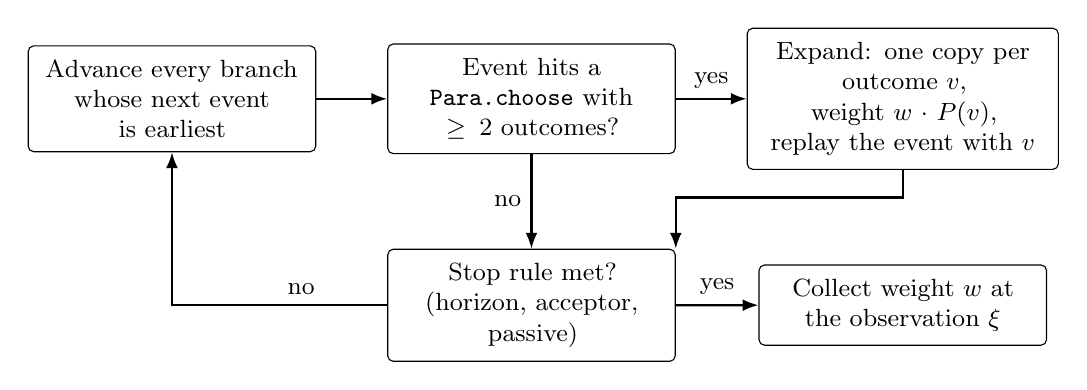
\begin{tikzpicture}[node distance=7mm and 9mm]
\node[box,text width=3.3cm] (adv) {Advance every branch\\whose next event\\is earliest};
\node[box,text width=3.3cm,right=of adv] (draw) {Event hits a\\\code{Para.choose} with\\$\ge 2$ outcomes?};
\node[box,text width=3.6cm,right=of draw] (exp) {Expand: one copy per\\outcome $v$, weight $w\cdot P(v)$,\\replay the event with $v$};
\node[box,text width=3.3cm,below=12mm of draw] (stop) {Stop rule met?\\(horizon, acceptor,\\passive)};
\node[box,text width=3.3cm,below=12mm of exp] (col) {Collect weight $w$ at\\the observation $\xi$};
\draw[flow] (adv) -- (draw);
\draw[flow] (draw) -- node[above,font=\small]{yes} (exp);
\draw[flow] (draw) -- node[left,font=\small]{no} (stop);
\draw[flow] (exp.south) -- ++(0,-0.35) -| (stop.north east);
\draw[flow] (stop) -- node[above,font=\small]{yes} (col);
\draw[flow] (stop.west) -| node[pos=0.2,above,font=\small]{no} (adv.south);
\end{tikzpicture}
\caption{The engine cycle. All branches share one simulation clock. Branching takes no simulated time.}
\label{fig:loop}
\end{figure}

\paragraph{What you get back.} A \code{ParaResult}: the weighted distribution of terminal observations
(\code{distribution()}), expectations of any function of the observation (\code{expectation(f)}), distributions of a
summary (\code{marginal(g)}), the omitted probability when you prune (\code{residual()}), and run statistics (\code{stats()}).

%=====================================================================
\section{Setup}

\subsection{Requirements}
\begin{itemize}
\item JDK 17 or newer (\code{java} and \code{javac} on the \code{PATH}); Git Bash for the scripts.
\item The MS4 DEVS core. Two sources work:
  \begin{itemize}
  \item the core \emph{sources} bundled in \path{Binghamton/Demo Deliverable/ParaDEVS/src/com}, which need no MS4 Me
    installation and are used by default, or
  \item the MS4 Me 1.5 jars in \path{C:\Program Files\MS4 Systems\MS4 Me\plugins}, which are needed for code generated by
    MS4 Me (Section~\ref{sec:import}).
  \end{itemize}
\end{itemize}

\subsection{Folder layout}
\begin{center}
\begin{tabularx}{\linewidth}{@{}>{\ttfamily\small}l Y@{}}
\toprule
\normalfont\textbf{Path (in \texttt{ParaDEVS\_Library/})} & \textbf{Contents}\\
\midrule
src/main/java/paradevs/ & Model API: \code{Para.choose}, \code{Law}\\
src/main/java/paradevs/engine/ & Engine, \code{ParaSpec}, \code{ParaResult}, selection rules, input trace, transducer\\
src/main/java/paradevs/ms4/ & MS4 integration: coordinator, snapshots, merge keys\\
src/examples/java/examples/ & \code{tutorial/}, \code{reward/}, \code{finance/}, \code{baseball/} with their tests\\
src/sandbox/java/sandbox/ & Staging area for your experiments (template: \code{RandomWalk}, \code{RunSandbox})\\
lib/ms4-core.jar & MS4 core packaged from Demo Deliverable, used by VS Code\\
.vscode/ & VS Code settings, run configurations and tasks\\
src/ms4me\_import\_demo/java/ & JobProcessorExample imported from MS4 Me (Section~\ref{sec:import})\\
scripts/ & \code{build\_library.sh}, \code{run\_my\_model.sh}, \code{run\_ms4me\_import\_demo.sh}\\
notes/ & Design notes; \code{05\_library\_v0.md} describes the implementation\\
docs/howto/ & This guide\\
\bottomrule
\end{tabularx}
\end{center}

\subsection{Build and run the tests}
From the \code{ParaDEVS\_Library} folder:
\begin{lstlisting}[style=plain]
bash scripts/build_library.sh             # build, then run every test
bash scripts/build_library.sh tutorial    # one test: sandbox | tutorial | reward | finance | baseball | plain
\end{lstlisting}
Each test prints \code{PASS}/\code{FAIL} lines and a tally. The full suite currently passes 77 checks: the tutorial
against a hand answer, the paper's timed reward example against exact rational results, finance against the Demo
Deliverable baseline, and baseball against the original BaseballDEVS\_v7 engine.

\subsection{Run your own model}
Put your \code{.java} files in any folder (any package layout) and give the class that has \code{main}:
\begin{lstlisting}[style=plain]
bash scripts/run_my_model.sh path/to/my/src  mymodels.RunMyModel           # bundled core
bash scripts/run_my_model.sh path/to/my/src  mymodels.RunMyModel --ms4me   # MS4 Me jars
\end{lstlisting}
The script compiles the MS4 core, the library and your folder together into \path{build/user}, then runs your class.

\subsection{Working in VS Code}
\label{sec:vscode}
VS Code is the current environment for testing. Open the \code{ParaDEVS\_Library} folder itself (File $\to$ Open
Folder) with the Java Extension Pack installed. The folder is preconfigured:
\begin{itemize}
\item \textbf{Sources and classpath} (\path{.vscode/settings.json}): \path{src/main/java}, \path{src/examples/java} and
  \path{src/sandbox/java}, plus \path{lib/ms4-core.jar}. Exactly this configuration compiles cleanly from the
  command line. If the editor shows errors on first open, run ``Java: Clean Java Language Server Workspace''.
\item \textbf{Run and Debug} (\path{.vscode/launch.json}): \emph{Sandbox: RunSandbox}, \emph{Run current file}, the
  tutorial, each \code{Verify*} test, and a plain MS4 run. All run with the library folder as the working directory,
  so relative data paths work exactly as in the scripts. Each target was run with this classpath and working
  directory, and all pass. Use the Debug variant to set breakpoints in model code or in the engine.
\item \textbf{Tasks} (Terminal $\to$ Run Task, run in Git Bash): build and run all tests, run one test, package
  the MS4 core jar, the MS4 Me import demo, and compile this guide.
\end{itemize}
\textbf{Where to put new work:} \path{src/sandbox/java/sandbox/}. The template there is a random walk whose next step is
drawn on state entry. \code{RunSandbox} checks it against the binomial law and shows safe merging shrinking 64 leaves
to 12. Copy the two files, rename them, and start from there. When a model is worth keeping, move it under
\path{src/examples} with a test.

\note{The MS4 Me import demo is not on the VS Code source path, because it needs the MS4 Me jars, which would clash
with \path{lib/ms4-core.jar}. Run it with its task. If the Demo Deliverable core sources change, rerun the
\emph{package MS4 core jar} task.}

%=====================================================================
\section{Key ideas in one page}

\begin{center}
\begin{tabularx}{\linewidth}{@{}>{\bfseries}p{3.1cm} Y@{}}
\toprule
Term & Meaning\\
\midrule
Draw (choice point) & A call to \code{Para.choose(label, law)} with at least two possible outcomes. Laws with one outcome never branch.\\
\code{Law} & A finite list of (value, probability) pairs. It must sum to 1 (within $10^{-6}$). Zero-probability values are dropped.\\
Departure & One DEVS event of the top model: internal, external (input), or confluent (both). Draws happen inside departures, including in \code{initialize()}.\\
Branch & One copy of the run: model state, clock, position in the input trace, entry count, observation $\xi$, weight $w$.\\
Persistent entry & A completed state after a departure. The initial state is entry 1.\\
Input trace & A fixed list of timed messages sent to the top model's input ports.\\
Transducer & Folds the top model's \emph{outputs} into the observation $\xi$ (e.g.\ ``number of jobs done''). $\xi$ must be immutable with \code{equals}/\code{hashCode}.\\
Stop rules & A branch ends at the \emph{horizon} (entry count $m$), when an \emph{acceptor} returns true, or when it is \emph{passive} (no event scheduled and no inputs left).\\
Selection rule & What to do at a draw: \emph{exhaustive} (all outcomes), \emph{Monte Carlo} (one sampled outcome), \emph{partial} (outcomes above a threshold), or \emph{hybrid} (a rule per label).\\
Safe merge & Two new branches with identical complete state and identical $\xi$ are combined, and their weights added. This never changes the result.\\
Residual & Probability left unexplored by partial selection. True probabilities lie between the result and result $+$ residual.\\
\bottomrule
\end{tabularx}
\end{center}

\paragraph{There is no ``step''.} The old tree engines worked in steps: one tree level, one outcome forced in from
outside, one simulation run, one state save, all at once. The library separates these. Time advances one DEVS event
(departure) at a time. Branching happens only where the model calls \code{Para.choose}. An event may make no draw (no
branching), one draw, or several, and a later draw may depend on an earlier one in the same event. There is no
\code{depth}: a run ends by its stop rules. See the \doclink{architecture/ParaDEVS_Architecture.pdf}{Architecture Guide}, Section ``Step versus draw''.

\note{The engine observes only what leaves the top model through its output ports. If you care about internal
state, such as cash or a queue length, have a component report it on an output port and couple that port out (both
tutorials do this).}

\paragraph{The one rule for models.} Given the state, the event, and the values returned by \code{Para.choose}, a
model's transition must be \emph{deterministic}. The engine replays an event with the chosen values to continue
a branch, so the model must ask for the same draws in the same order. Do not use \code{Math.random}, \code{Random},
wall-clock time, or the iteration order of \code{HashSet}/\code{HashMap} over objects without \code{equals}.

%=====================================================================
\section{Tutorial 1: a DEVS model built purely in Java}
\label{sec:tutorial}

We build a single server with no waiting room. Customers arrive at times 1, 2 and 3. The server takes 0.5 time units
with probability 0.6 or 1.5 with probability 0.4. A customer who arrives while the server is busy is lost. Question:
\emph{how many customers are served?} The whole model is in \path{src/examples/java/examples/tutorial/}.

\subsection{The answer by hand}
\begin{figure}[h]
\centering
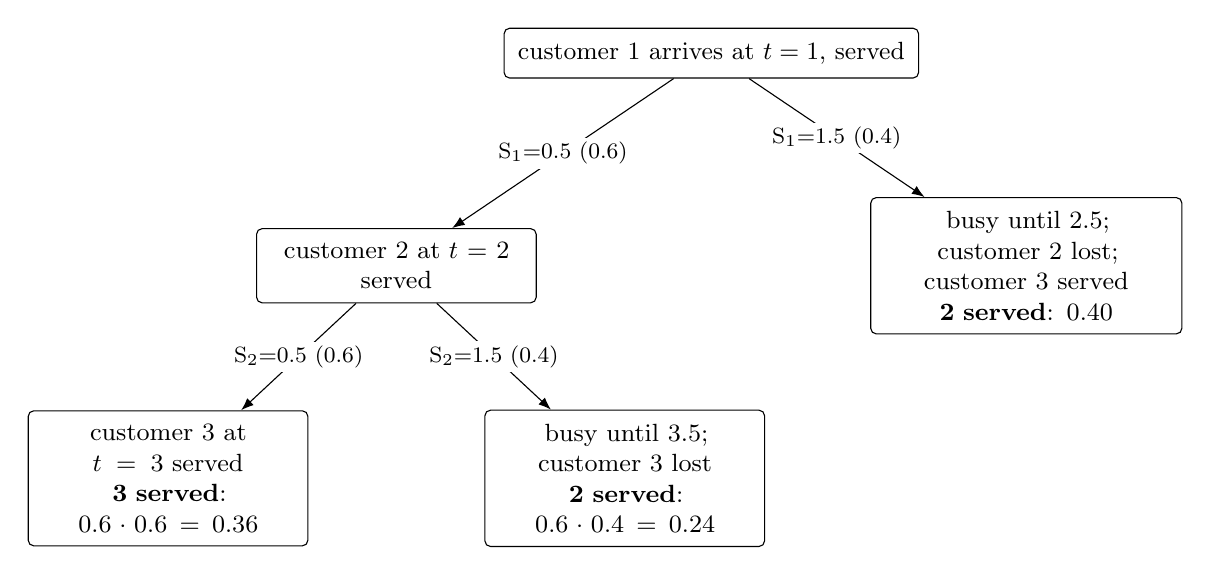
\begin{tikzpicture}[level distance=27mm, every node/.style={font=\small},
  level 1/.style={sibling distance=80mm}, level 2/.style={sibling distance=58mm},
  edge from parent/.style={draw,-{Latex[length=1.6mm]}},
  lbl/.style={midway,fill=white,inner sep=1.5pt,font=\footnotesize}]
\node[box] {customer 1 arrives at $t=1$, served}
  child { node[box,text width=3.2cm] {customer 2 at $t=2$\\served}
    child { node[box,text width=3.2cm] {customer 3 at $t=3$ served\\\textbf{3 served}: $0.6\cdot0.6=0.36$} edge from parent node[lbl] {S$_2$=0.5 (0.6)} }
    child { node[box,text width=3.2cm] {busy until 3.5;\\customer 3 lost\\\textbf{2 served}: $0.6\cdot0.4=0.24$} edge from parent node[lbl] {S$_2$=1.5 (0.4)} }
    edge from parent node[lbl] {S$_1$=0.5 (0.6)} }
  child { node[box,text width=3.6cm] {busy until 2.5; customer 2 lost;\\customer 3 served\\\textbf{2 served}: $0.40$} edge from parent node[lbl] {S$_1$=1.5 (0.4)} };
\end{tikzpicture}
\caption{The tree the engine will explore. Customer 3's own service time also branches, but does not change the count.}
\label{fig:tree}
\end{figure}

So $P(\text{3 served}) = 0.6 \times 0.6 = 0.36$, $P(\text{2 served}) = 0.64$, and $E[\text{served}] = 2.36$.
The tree has 5 leaves: customer 3's service time adds a split in two places.

\subsection{Step 1: write the atomic model}
An MS4 atomic model extends \code{AtomicModelImpl} and overrides the four DEVS functions:
\code{getTimeAdvance} ($ta$), \code{getOutput} ($\lambda$), \code{internalTransition} ($\delta_{int}$) and
\code{externalTransition} ($\delta_{ext}$). \code{confluentTransition} defaults to internal, then external.
Ports are created with \code{addInputPort}/\code{addOutputPort}. The only paratemporal-specific code is the
\code{SERVICE} law and the \code{Para.choose} call in \code{externalTransition}.

\lstinputlisting[caption={\code{Server.java}: the complete atomic model},label=lst:server]{\src/examples/java/examples/tutorial/Server.java}

Points to notice:
\begin{itemize}
\item State lives in fields (\code{phase}, \code{current}, \code{sigma}) and is set in \code{initialize()}, which the
  engine calls at time 0. Do not rely on field initializers for state that \code{initialize()} should reset.
\item \code{sigma -= e} keeps the remaining service time when a customer is lost. That is standard MS4 style.
\item Fields must be \code{Serializable}: the engine copies branches by serialization. Primitives, strings, arrays and
  your own \code{Serializable} classes are fine.
\end{itemize}

\subsection{Step 2: run it with an input trace}
To run the server alone, customers come from an input trace. The port name in the trace is the name given to
\code{addInputPort} (here \code{"customer"}). The transducer counts \code{done} outputs; that count is the observation.

\lstinputlisting[linerange={23-30,36-39},caption={Transducer and the first engine run (from \code{RunServiceLine.java})}]{\src/examples/java/examples/tutorial/RunServiceLine.java}

Output:
\begin{lstlisting}[style=plain]
Step 1  Server + input trace
    served=2  status=PASSIVE  weight=0.6400
    served=3  status=PASSIVE  weight=0.3600
    E[served]=2.3600  mass=1.0000  leaves=5 choiceNodes=4 departures=23 merged=0 maxLive=5 ms=68
\end{lstlisting}
That is the hand answer, with 5 leaves and 4 draws expanded. \code{PASSIVE} means each branch ended because the server
was idle and no inputs were left, so no horizon was needed.

\subsection{Step 3: make it a coupled model}
Now generate the customers inside the model. \code{Arrivals} is a deterministic atomic model, and \code{ServiceLine}
couples the two. This is exactly what an SES would declare.

\lstinputlisting[firstline=8,caption={\code{Arrivals.java} (class body)}]{\src/examples/java/examples/tutorial/Arrivals.java}
\lstinputlisting[firstline=6,caption={\code{ServiceLine.java}: the coupled model}]{\src/examples/java/examples/tutorial/ServiceLine.java}

The engine runs coupled models with the same call; no trace is needed now:
\begin{lstlisting}
ParaResult<Integer> coupled = ParaEngine.run(ParaSpec.of(() -> new ServiceLine(3), SERVED));
\end{lstlisting}
\begin{lstlisting}[style=plain]
Step 2  ServiceLine (coupled)
    served=2  status=PASSIVE  weight=0.6400
    served=3  status=PASSIVE  weight=0.3600
    E[served]=2.3600  mass=1.0000  leaves=5 choiceNodes=4 departures=23 merged=0 maxLive=5 ms=33
\end{lstlisting}

\note{Pass a \emph{factory} (\code{() -> new ServiceLine(3)} or \code{Server::new}), not a model instance. The engine
builds the model once, then copies it.}

\subsection{Step 4: options}
\begin{lstlisting}
ParaSpec.of(() -> new ServiceLine(3), SERVED).merge(ParaSpec.Merge.SAFE);         // safe merging
ParaSpec.of(() -> new ServiceLine(3), SERVED)
        .selection(SelectionRule.monteCarlo()).roots(2000).seed(11);               // Monte Carlo
ParaSpec.of(() -> new ServiceLine(3), SERVED)
        .selection(SelectionRule.partialExhaustive(0.5));                          // prune outcomes < 0.5
\end{lstlisting}
\begin{lstlisting}[style=plain]
Step 4  ServiceLine, Monte Carlo N=2000
    served=2  status=PASSIVE  weight=0.6465
    served=3  status=PASSIVE  weight=0.3535
    E[served]=2.3535  mass=1.0000  leaves=2000 choiceNodes=4707 departures=17414 ...
\end{lstlisting}
Monte Carlo gives an unbiased estimate, here within one standard error of 0.36. Safe merging finds nothing to merge in
this model, because no two branches have the same state at the same time. In the baseball example it cuts 24{,}450
leaves to 195.

\subsection{Step 5: it is still an ordinary MS4 model}
\begin{lstlisting}
Para.setDefaultRandom(new Random(3));      // optional: reproducible sampling
Simulation sim = new SimulationImpl("plain run", new ServiceLine(3));
sim.startSimulation(0);
sim.simulateIterations(Long.MAX_VALUE);
\end{lstlisting}
With no engine active, \code{Para.choose} samples, and MS4 runs one random path.

\subsection{Step 6: test it}
A model is ready when these hold. \code{RunServiceLine} checks all of them:
\begin{enumerate}
\item Exhaustive \code{totalMass()} is 1 (up to rounding in your data).
\item The result matches a case you can work out by hand (as in Figure~\ref{fig:tree}).
\item Safe merging gives the same distribution as no merging.
\item Monte Carlo agrees with exhaustive within about 3--4 standard errors, $\sqrt{p(1-p)/N}$.
\item The plain MS4 run completes.
\end{enumerate}
Run it with \code{bash scripts/build\_library.sh tutorial}; it ends with \code{10 passed, 0 failed}.

\paragraph{Try next.} Change \code{ServiceLine(3)} to \code{ServiceLine(8)} and watch the leaf count grow. Add a
second outcome law in \code{Arrivals} (random inter-arrival times). Or add an output port reporting lost customers
and count both in the transducer.

%=====================================================================
\section{Tutorial 2: bringing a model over from MS4 Me}
\label{sec:import}

MS4 Me turns DNL into Java atomic models and turns SES/PES into a Java coupled model. The engine runs that Java
directly. This section uses the \code{JobProcessorExample} project from the MS4 Me workspace; the result is in
\path{src/ms4me_import_demo/java}.

\subsection{What to bring over}
\begin{center}
\begin{tabularx}{\linewidth}{@{}>{\raggedright\arraybackslash\ttfamily\small}p{4.9cm} Y >{\raggedright\arraybackslash\small}p{2.3cm}@{}}
\toprule
\normalfont\textbf{From the MS4 Me project} & \textbf{What it is} & \textbf{Needed?}\\
\midrule
src/Models/java/\newline <Atomic>.java & Java generated from each \code{.dnl} & \textbf{yes}\\
src/Models/java/\newline <Coupled>.java & Coupled model written by the PES (\code{write class files}); its \code{make()} holds \code{addChildModel}/\code{addCoupling} & \textbf{yes} (or write the couplings yourself)\\
src/Models/java/\newline <Data>.java & Message and data classes (e.g.\ \code{WorkToDo}, \code{Players}) & \textbf{yes}\\
src/Models/txt/*.csv & Input data the models read & if used\\
src/Models/dnl, ses, pes & Specifications & no (keep them for regeneration)\\
Run*, GeneralTree, GeneralNode, SimulateModel, SimResult & The old hand-built tree engine & \textbf{no}: the library replaces it\\
\bottomrule
\end{tabularx}
\end{center}
Keep the package name (\code{Models.java}) as generated, so you don't have to edit every file.

\subsection{Pick a build route}
Generated MS4 Me files import \code{SimViewer} and \code{SimulationOptionsImpl} for their \code{main()} methods.
Those two classes are in the MS4 Me jars but not in the bundled core.
\begin{center}
\begin{tabularx}{\linewidth}{@{}>{\bfseries}p{3.4cm} Y Y@{}}
\toprule
Route & Use when & Command\\
\midrule
A. MS4 Me jars & MS4 Me is installed; files stay as generated & \code{run\_my\_model.sh <dir> <Main> -{}-ms4me}\\
B. Bundled core & No MS4 Me installation; you can edit the files & delete each generated \code{main()} and its \code{SimViewer}/\code{helpers} imports, then \code{run\_my\_model.sh <dir> <Main>}\\
\bottomrule
\end{tabularx}
\end{center}
Route B is what the Demo Deliverable did: its generated \code{main()} methods are commented out.

\subsection{The edits}
\begin{enumerate}[label=\textbf{E\arabic*.}]
\item \textbf{Replace every random draw by \code{Para.choose}.} Search for \code{Math.random}, \code{new Random},
  \code{nextDouble}, \code{nextInt}, and any sampling helper. Inside DNL code blocks, use fully qualified names so no
  import is needed:
\begin{lstlisting}
paradevs.Para.choose("processingTime",
    paradevs.Law.of(java.util.Arrays.asList(5.0, 15.0), new double[] {0.7, 0.3}))
\end{lstlisting}
\item \textbf{Expose what you want to measure.} The engine sees only the top model's outputs. Add an output port to
  the coupled model and couple the interesting component port to it (\code{addCoupling(child.outX, addOutputPort("x", T.class))}).
\item \textbf{Move the starting state into \code{initialize()}.} The old engines injected state by reflection
  (\code{setValue(cm, "Portfolio", "Shares", ...)}, \code{Portfolio.phase = cState}). Under the library, the model starts
  from \code{initialize()} and evolves itself. Constructor parameters are fine for fixed data such as tables or prices.
\item \textbf{Move forced outcomes inside the model.} The old pattern set an outcome from outside
  (\code{setValue(cm,"HitMaker","HitType",outcome,...)}) and sent its probability through the message. Instead, the
  component that knows the situation draws the outcome itself:
\begin{lstlisting}
// before (HitMaker): outcome injected, probability sent along with it
//   if (HitType == "Single") { Prob = batter.getBattingProb()[1]; output.add(outSingle, ...); }
// after (Batter): the batter draws the outcome
hit = Para.choose("hit", Law.of(HITS, scoringPosition ? scoring[index] : normal[index]));
\end{lstlisting}
  If the law depends on another component's state (bases occupied, shares held), have that component report it on a
  coupling, as the finance and baseball examples do.
\item \textbf{Data classes:} make them \code{Serializable}. Give message and observation classes
  \code{equals}/\code{hashCode} if you want safe merging to find matches.
\end{enumerate}

\subsection{Worked example: JobProcessorExample}
The generator gives each job a processing time of \code{20 + count}. We make it 5 or 15 at random and observe solved
jobs. These are the only two edits in the generated files:
\begin{lstlisting}
// GeneratorOfJobs.java (in initialize() and in the internal transition)
// ParaDEVS: random processing time (was: wtd.setProcessingTime(20 + count);)
wtd.setProcessingTime(paradevs.Para.choose("processingTime",
    paradevs.Law.of(java.util.Arrays.asList(5.0, 15.0), new double[] {0.7, 0.3})));

// SimpleWorkFlow.java, end of make()
// ParaDEVS: expose solved jobs as a coupled-model output so the experiment can observe them
addCoupling(ProcessorOfJobs.outJob, addOutputPort("solved", WorkToDo.class));
\end{lstlisting}
The driver counts \code{solved} outputs and stops each branch at its first event at or after $t=45$ (an acceptor, since
the generator would otherwise run for 50 jobs):
\lstinputlisting[linerange={25-39},caption={Driver (from \code{demo/RunJobShop.java})}]{\src/ms4me_import_demo/java/demo/RunJobShop.java}
Run it with \code{bash scripts/run\_ms4me\_import\_demo.sh}:
\begin{lstlisting}[style=plain]
Exhaustive: leaves=42 choiceNodes=41 departures=163 merged=0 maxLive=32 ms=651
    solved by t=45: 2   P=0.2160
    solved by t=45: 3   P=0.5439
    solved by t=45: 4   P=0.2401
    E[solved]=3.0241  mass=1.0000
Monte Carlo N=2000: leaves=2000 ...
    solved by t=45: 2   P=0.2160
    solved by t=45: 3   P=0.5465
    solved by t=45: 4   P=0.2375
Plain MS4 run completed 200 iterations.
\end{lstlisting}
Check: four jobs are solved by $t=45$ only if all four processing times are short, $0.7^4 = 0.2401$. The first job's
time is drawn inside \code{initialize()}, and the engine branches there too.

\subsection{Port names in generated code}
DNL \code{accepts input on Job} creates a port named \code{inJob}, and \code{generates output on Job} creates \code{outJob}.
Use those names in input traces and transducers (\code{InputTrace.builder().at(5.0, "inJob", job)}).

\subsection{Keeping MS4 Me in sync}
If you regenerate Java from DNL, edits made only in the Java are lost. Put the \code{Para.choose} call in the DNL code
block (fully qualified, as in E1), and copy \path{src/main/java/paradevs} into the MS4 Me project's \code{src} folder so
the generated code compiles there.

\note{The two steps in this subsection have not yet been tried inside the MS4 Me IDE. Everything else in this section
was run as shown.}

\subsection{Testing an imported model}
Use the checklist of Tutorial~1, Step 6, plus one more test when an old result exists. The finance and baseball tests
are complete templates (\path{src/examples/java/examples/finance/VerifyFinance.java},
\path{.../baseball/VerifyBaseball.java}). The approach:
\begin{itemize}
\item Run the old project once and save its output (a CSV of probabilities or expected values).
\item Run the library exhaustively and map each terminal observation to the old summary with \code{marginal(g)}, e.g.\
  shares held, or (bases, outs, runs).
\item Compare probabilities to about $10^{-12}$ and money or runs to about $10^{-6}$.
\end{itemize}
The old IH engines merged branches by a summary and added their weights. Because that merge is linear, the library's
exact distribution reproduces those numbers through \code{marginal}, without any IH merging.

%=====================================================================
\section{API reference}

\subsection{Model side}
\begin{center}
\begin{tabularx}{\linewidth}{@{}>{\ttfamily\small}p{6.6cm} Y@{}}
\toprule
\normalfont\textbf{Call} & \textbf{Use}\\
\midrule
Para.choose(String label, Law<T> law) & Draw a value. The label names the primitive (used by hybrid selection and in error messages).\\
Law.of(v1, p1, v2, p2, ...) & Law from value/probability pairs. Avoid it when values are numbers too; use the list form.\\
Law.of(List<T> values, double[] probs) & Law from parallel arrays.\\
Law.of(Map<T, Number> probs) & Law from an ordered map.\\
Law.dirac(v) & A single certain value (never branches).\\
Law.asGiven(values, probs, tol) & Accept a total mass within \code{tol} of 1, to reproduce slightly improper source data.\\
Para.setDefaultRandom(Random r) & Seed the sampler used outside the engine.\\
\bottomrule
\end{tabularx}
\end{center}

\subsection{Experiment side: \code{ParaSpec}}
\begin{center}
\begin{tabularx}{\linewidth}{@{}>{\ttfamily\small}p{6.6cm} Y@{}}
\toprule
\normalfont\textbf{Builder call} & \textbf{Meaning (default)}\\
\midrule
ParaSpec.of(factory, transducer) & Model factory and observation (required).\\
.trace(InputTrace) & Fixed timed inputs (none).\\
.horizon(m) & Stop at the $m$-th persistent entry; the initial state is entry 1 (no limit).\\
.acceptor((xi, t, n) -> boolean) & Extra stopping rule on observation, time, entry count (none).\\
.selection(SelectionRule) & \code{exhaustive()} (default), \code{monteCarlo()}, \code{partialExhaustive(p)}, \code{hybrid(map, other)}.\\
.roots(N) & $N$ starting copies of weight $1/N$; use with Monte Carlo (1). Not combinable with safe merging (refused).\\
.merge(ParaSpec.Merge.SAFE) & Merge identical new branches (\code{NONE}).\\
.seed(s) & Seed for sampled selection (1).\\
.maxLive(n) & Abort if more than $n$ branches are live (5{,}000{,}000).\\
\bottomrule
\end{tabularx}
\end{center}
\code{InputTrace.builder().at(time, port, value)...build()}: messages at the same time are delivered together.
\code{Transducer.history()} records every output with its time; write your own (Tutorial 1) to keep a smaller summary,
which also merges better.

\subsection{Results: \code{ParaResult}}
\begin{center}
\begin{tabularx}{\linewidth}{@{}>{\ttfamily\small}p{5.0cm} Y@{}}
\toprule
\normalfont\textbf{Method} & \textbf{Returns}\\
\midrule
distribution() & Map from (observation $\xi$, stop status) to total weight.\\
expectation(f) & $\sum w\,f(\xi)$: expected value of a function of the observation.\\
marginal(g) & Distribution of $g(\xi)$, with weights of equal images summed.\\
totalMass() & Sum of weights; 1 for exhaustive runs with proper laws.\\
residual() & Omitted probability from partial selection.\\
stats() & \code{leaves} (finished branches), \code{choiceNodes} (draws expanded), \code{departures} (event runs incl.\ replays), \code{merged}, \code{maxLive}, \code{ms}.\\
\bottomrule
\end{tabularx}
\end{center}

%=====================================================================
\section{Troubleshooting}
\begin{center}
\small
\begin{tabularx}{\linewidth}{@{}>{\raggedright\arraybackslash}p{4.6cm} >{\raggedright\arraybackslash}X@{}}
\toprule
\textbf{Message or symptom} & \textbf{Cause and fix}\\
\midrule
\code{Law mass must be 1 (got ...)} & Probabilities do not sum to 1. Fix the data, or use \code{Law.asGiven(..., tol)} on purpose.\\
\code{Replay mismatch at draw '...'} or \code{Replay used k of m supplied values} & The event is not deterministic given its state: other randomness, time-of-day, or hash-order iteration. Make all randomness go through \code{Para.choose}.\\
\code{choose() called after a suspension} & Model code catches \code{Throwable}/\code{Error} around a draw. Let \code{Para.Suspension} pass through.\\
\code{Model state is not serializable} & A field's class is not \code{Serializable}. Make it so. Use \code{transient} only for caches that can be rebuilt.\\
\code{Model ... has no input port ...} & Trace port name differs from the model's port. Generated ports are named \code{inX}/\code{outX}.\\
\code{Live branches exceed maxLive} & The tree is too large. Use a horizon or acceptor, safe merging, Monte Carlo, or partial selection.\\
Result empty or every observation \code{null} & Nothing reaches the top model's outputs. Couple the port out (E2) and check the transducer's port name.\\
Merging never merges & $\xi$ lacks \code{equals}/\code{hashCode}, $\xi$ is a full history, or the state really differs (e.g.\ different times).\\
\code{Model failed during INIT ...} & An exception in model code. Note that \code{initialize()} runs at time 0.\\
Very slow run & Count \code{departures}: each draw replays its event. Merge, shorten the horizon, or sample.\\
\bottomrule
\end{tabularx}
\end{center}

%=====================================================================
\section{Scope of v0 and further reading}
\begin{itemize}
\item Supported: atomic and coupled MS4 models, fixed input traces, horizon/acceptor/passive stopping, exhaustive,
  Monte Carlo, partial and hybrid selection, safe merging.
\item Not yet: deferred output draws (the paper's $ps$ representation), inputs that react to outputs (e.g.\ an RL agent),
  parallel execution, exhaustive treatment of continuous laws (sample them instead).
\item The engine follows \path{Do s/documents/paratemporal/main_paratemporal.tex}; the replay mechanism is the
  ``derandomized departure'' of \path{Paratemporal_Adaptation.tex}. Implementation notes and the verification record
  are in \path{notes/05_library_v0.md}.
\end{itemize}

\end{document}
